\documentclass[a4paper,10pt]{scrartcl}
\usepackage[utf8]{inputenc}
\usepackage{graphicx}
\usepackage[left=2cm,right=2cm,top=2cm,bottom=2cm]{geometry}
%opening
\title{MVDBS:Knotenspeicherung im MongoDB}
\author{Roland Hediger}

\begin{document}

\maketitle

\begin{abstract}

\end{abstract}

\section{Storage Model}
 MongoDB speichert daten als Dokumente in eine Binäre Darstellung (Binary JSON) - BSON.
 BSON erweitert JSON damit es mehrere Typen einschliesst wie int,long, und float. BSON Dokumente beinhalten ein oder 
mehrere Felder und jedes Feld beinhaltet der Wert von einem spezifischen Datentyp : Arrays,Binärdaten,und 
Unterdokumenten. Dokumeten haben eine ähnliche Struktur und sind in Sammelungen oder Collections organisiert. Es ist 
hilfreich , die Collections als Tabellen-ähnliche Strukturen vorzustellen. Dokumenten sind dann nach deiser Vorstellung 
wie Zeilen und die Felder ähnlich wie Spalten.

\subsection{BSON Spezifikation}
MongoDB Dokumenten haben folgenden Struktur:
\begin{verbatim}
 {
   field1: value1,
   field2: value2,
   field3: value3,
   ...
   fieldN: valueN
}
\end{verbatim}

BSON Dokumente sind aber limitiert in der Grösse bis zum 16MB.
\section{Datenstruktur}

Jede MongoDB Knoten hat ein Namespace Datei,Journal Datei, und Dateien für Daten.
Dateien mit Daten speichern BSON Dokumente ,indexes, und MongoDB Metadata in speziellen Strukturen die Extents heissen.
Jede Daten-Datei ist aus mehrere Extents zusammengestellt.

\subsection{Beziehung zwischen Daten und Extents}
\begin{figure}[h!]
 \centering
 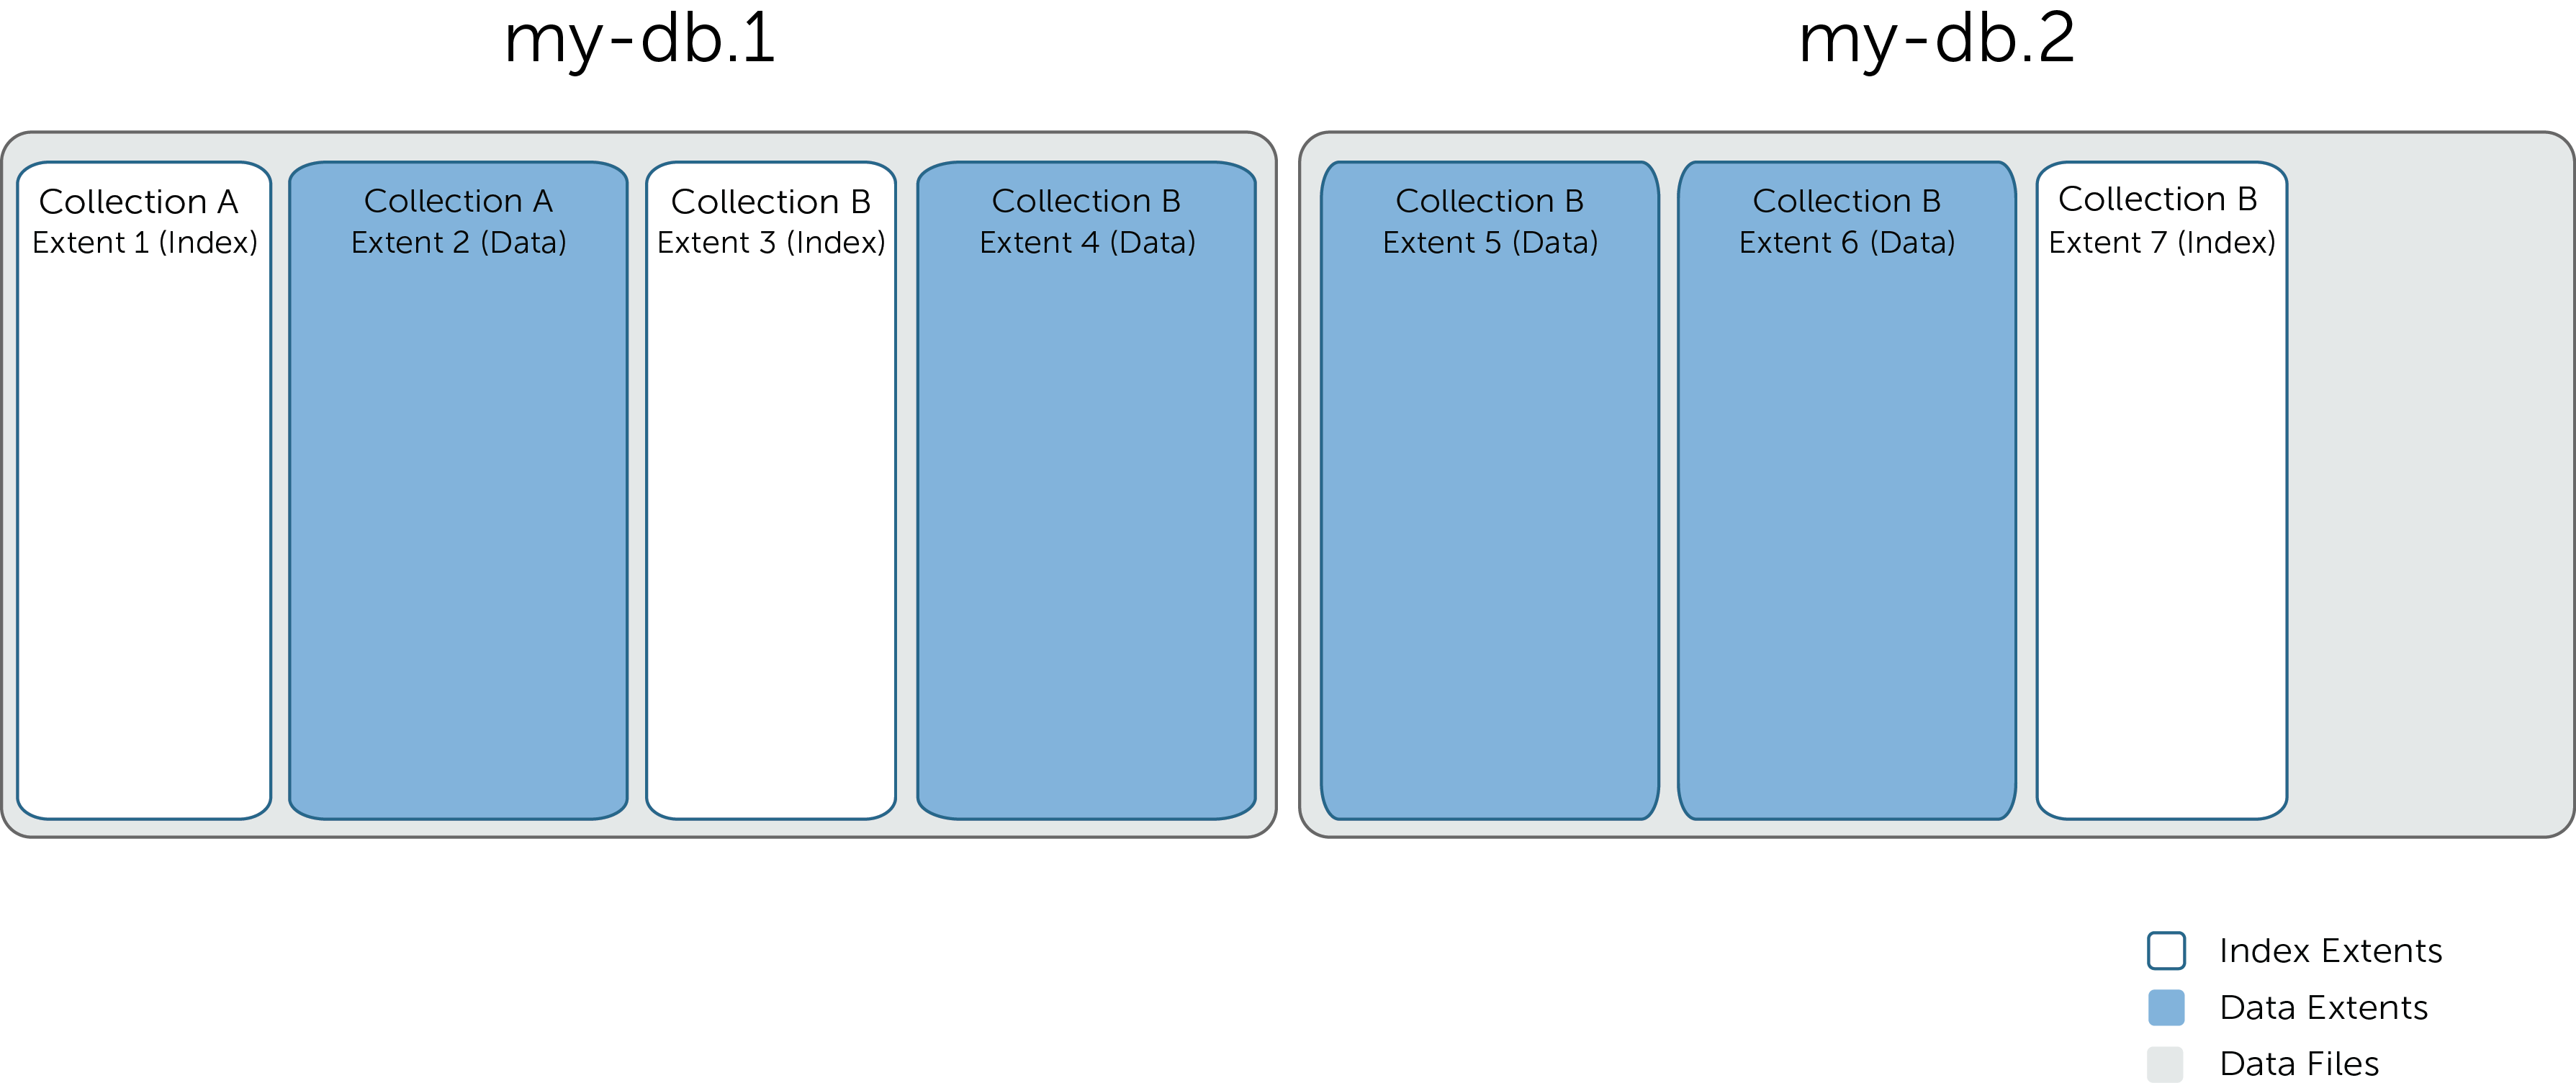
\includegraphics[scale=0.4]{./de.png}
 % de.png: 3578x1504 pixel, 300dpi, 30.29x12.73 cm, bb=0 0 859 361
\caption{http://blog.mongolab.com/2014/01/how-big-is-your-mongodb/}
 \end{figure}

\begin{itemize}
 \item Daten und indexen (indices)  haben beide seperaten Mengen von Extents
 \subitem Kein Extent hat Informationen über mehr als eine Collection.
 \item Data und Indexes gehen über mehrere Extents hinaus.
 \item MongoDB versucht immer zuerst die freien Platz innerhalb existierenden Extents auszunutzen bevor eine neue 
erzeugt wird.
\end{itemize}

\subsection{Speicherung Metriken}
\begin{description}
 \item [dataSize]
Innherhalb Collections sind Dokumenten mit Padding alloziert, das heisst der Behalter ist etwas grösser als die 
tätsächlich abgespeicherte Daten vom Dokument. Die grösse des Dokuments wird immer inklusiv Padding gemessen.
\item [fileSize] Gesamtgrösse von alle Extents. Extents sind wie Dokumente mit Padding alloziert.Logischerweise ist 
dieses Metrik immer grösser als datasize.
\end{description}
\begin{figure}[h!]
 \centering
 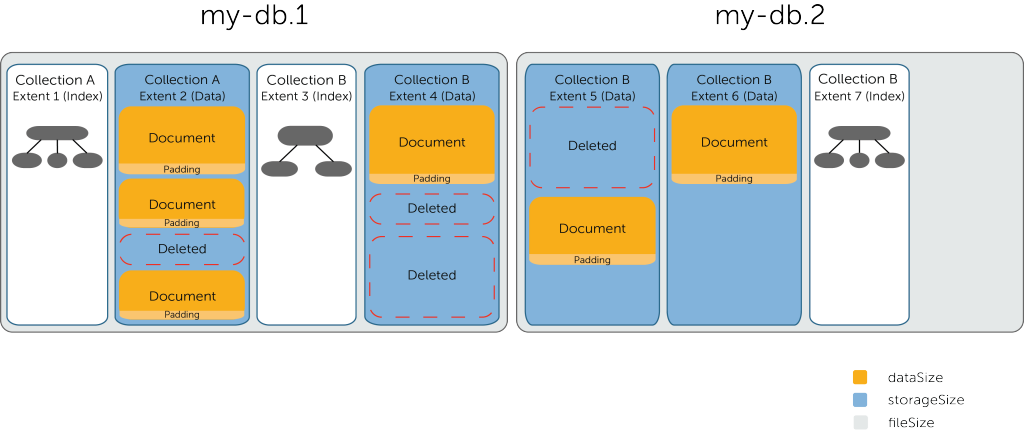
\includegraphics[scale=1]{./de2.png}
 % de.png: 3578x1504 pixel, 300dpi, 30.29x12.73 cm, bb=0 0 859 361
\caption{http://blog.mongolab.com/2014/01/how-big-is-your-mongodb/}
 \end{figure}

\section{GridFS}
Statt ein grosserer Datei innerhalb von ein Dokument abzuspeichern, teilt Gridfs der Datei auf in ``Chunks'' und 
speichert jede Chunk als seperates Dokument. Chickgrösse wird auf 255k limitiert. Es bunutzt dann zwei Collections eine 
für die Datenchunks und eine für die dazugehörige metadaten. 

Wenn man eine Query abschickt um dieser Datei zu hohlen, der Treiber wird die Chunks zusemmenstellen

Es ist auch möglich bestimmte Teile von dem Datei auszohohlen.

Each document in the chunks collection represents a distinct chunk of a file as represented in the GridFS store. Each 
chunk is identified by its unique ObjectId stored in its \_id field.

GridFS uses a unique, compound index on the chunks collection for the files\_id and n fields. The files\_id field 
contains the \_id of the chunk’s “parent” document. The n field contains the sequence number of the chunk. GridFS 
numbers all chunks, starting with 0. For descriptions of the documents and fields in the chunks collection,
\newpage

\begin{thebibliography}{9}

\bibitem{MongoDB Architecture Guide}
  A MongoDB Whitepaper\\
  MongoDB 2.6\\
\bibitem{How big is your MongoDB}
How big is your MongoDB\\
http://blog.mongolab.com/2014/01/how-big-is-your-mongodb/
\bibitem{gridfs}
Getting Started with MongoDB + Gridfs \\
http://learnmongo.com/posts/getting-started-with-mongodb-gridfs/
\bibitem{gridfs manual}
http://docs.mongodb.org/manual/core/gridfs/
\end{thebibliography}
\end{document}
